\section{Extended Rosenbrock function}
\label{sec:extended_rosenbrock_results}

The extended Rosenbrock function is a generalization of the Rosenbrock function to $n$ dimensions, defined as follows.
Figure \ref{fig:extended_rosenbrock_surf} shows the surface plot of the 2-dimensional extended Rosenbrock function: notice that for $n=2$ it is identical to the standard Rosenbrock function, except for the $\frac12$ term.
\begin{align}
\label{eq:extended_rosenbrock}
F(x) &= \frac12 \sum_{k=1}^n f_k^2(x), &
f_k(x) &= \left \{ \begin{array}{ll}
10(x_k^2 - x_{k+1}), & k\mod 2 = 1\\
x_{k-1} -1, & k\mod 2 = 0
\end{array} \right .
\end{align}
The minimum of the function is in a very flat valley which is easy to reach, but in practice it's harder to converge to a minimum, which makes the extended Rosenbrock function a challenging optimization problem.

\begin{figure}
    \centering
    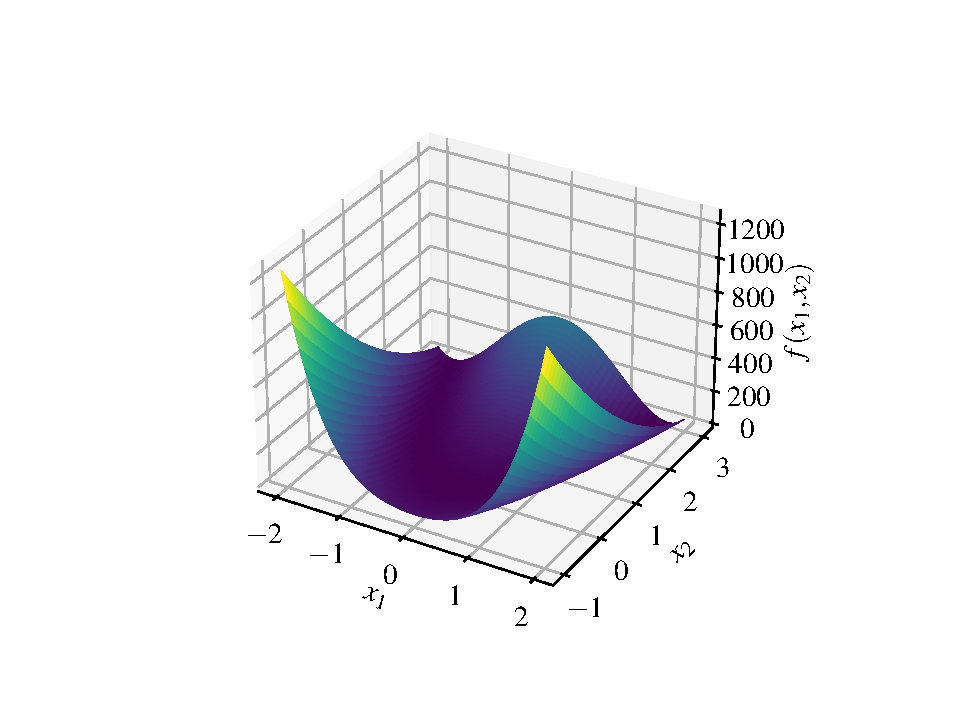
\includegraphics[width=0.5\textwidth]{figures/extended_rosenbrock_surf.pdf}
    \caption{Surface plot of the 2-dimensional extended Rosenbrock function}
    \label{fig:extended_rosenbrock_surf}
\end{figure}

\subsection{Exact gradient and Hessian}

The gradient of the extended Rosenbrock function is given by the following expression,
\begin{equation}
    \frac{\partial F}{\partial x_k} = 
    \left \{ \begin{array}{ll}
    200(x_k^3 - x_kx_{k+1}) + (x_k - 1), & k\mod 2 = 1\\
    -100(x_{k-1}^2 - x_k), & k\mod 2 = 0
    \end{array} \right .
\end{equation}
computation can be eased considering that component $k$ depends only on $f_k$ and $f_{k+1}$ when $k$ is odd, and only on $f_{k-1}$ when $k$ is even.
The Hessian of the extended Rosenbrock function is given by the following expression.
\begin{equation}
    \frac{\partial^2 F}{\partial x_k \partial x_j} = 
    \left \{ \begin{array}{ll}
    200(3x_k^2 - x_{k+1}) + 1, & j = k,\ k\mod 2 = 1\\
    100, & j = k,\ k\mod 2 = 0\\
    -200x_k, & \lvert k-j \rvert = 1,\ k\mod 2 = 1\\
    0, & \text{otherwise}
    \end{array} \right .
\end{equation}
Notice that the Hessian is a sparse matrix, with only $n$ non-zero elements on the diagonal and $n/2$ non-zero elements on the first co-diagonal.

\subsection{Finite differences gradient and Hessian}

When applying \ref{eq:findiff_gradient}, one can notice that the terms $F(x + he_k)$ and $F(x-he_k)$ only differ by terms $f_k$ and $f_{k+1}$ for $k$ odd, by terms $f_{k-1}$ for $k$ even.
Then to make function evaluations less expensive, we can define the following function $F_{\textit{fd},\,k}$, which can be plugged in \ref{eq:findiff_gradient} in place of $F$ yielding the same result.
\[
F_{\textit{fd},\,k}(x) = \left \{ \begin{array}{ll}
\frac12 f_k^2(x) + \frac12 f_{k+1}^2(x), & k\mod 2 = 1\\[.1cm]
\frac12 f_{k-1}^2(x), & k\mod 2 = 0
\end{array} \right .
\]
The same procedure can be applied for the Hessian, considering that:
\begin{itemize}
    \item entry $h_{k,k}$ depends only on $f_k$ and $f_{k+1}$ for $k$ odd, and only on $f_{k-1}$ for $k$ even;
    \item entry $h_{k,k+1}$ depends only on $f_k$ and $f_{k+1}$ for $k$ odd.
\end{itemize}
Then to make function evaluations less expensive, we can define the functions $F_{\textit{fd},\,k,k}$ and $F_{\textit{fd},\,k,k+1}$, which can be plugged in \ref{eq:findiff_hessian} in place of $F$ yielding the same result to compute entries $h_{k,k}$ and $h_{k,k+1}$ respectively.
\begin{align*}
F_{\textit{fd},\,k,k}(x) &= \left \{ \begin{array}{ll}
\frac12 f_k^2(x) + \frac12 f_{k+1}^2(x), & k\mod 2 = 1\\[.1cm]
\frac12 f_{k-1}^2(x), & k\mod 2 = 0
\end{array} \right .\\
F_{\textit{fd},\,k,k+1}(x) &= \left \{ \begin{array}{ll}
\frac12 f_k^2(x) + \frac12 f_{k+1}^2(x), & k\mod 2 = 1\\[.1cm]
0, & k\mod 2 = 0
\end{array} \right .
\end{align*}
Carefully applying perturbations and properly defining some helper functions, computations for both gradient and Hessian can be vectorized, making the implementation efficient.